\documentclass[a4paper,12pt]{article}
\usepackage[portuguese]{babel}
\usepackage{amsmath,amsthm,amssymb,mathtools,tikz,graphicx,pgfplots,verbatim,fancyhdr}
\pagestyle{fancy}%Style of page
\setlength{\headsep}{0.5in}

\lhead{%Header left
	Universidade Federal da Para\'iba \\
	Discente: Jefferson Bezerra dos Santos\\
	Docente: Jos\'e Miguel Aroztegui Massera 
}

\title{Lista de EDO}
\date{\vspace{-5ex}}

\begin{document}
\maketitle\thispagestyle{fancy}
\textbf{Observa\c c\~ao:}\\
Em algumas partes do c\'odigo foram inseridas quebras de linha para que o c\'odigo fosse inserido na folha A4. Caso seja necess\'ario
verificar o funcionamento dos c\'odigos esses podem ser encontrados na pasta desse arquivo com a extens\~ao *m. \\

\textbf{1. Quest\~ao:}\\
O c\'odigo a seguir se refere a implementa\c c\~ao do m\'etodo de Taylor para q = 3.
\verbatiminput{taylor3.txt}
\newpage

\textbf{2. Quest\~ao:}\\
O c\'odigo a seguir se refere a resolu\c c\~ao do problema de valor inicial pelo m\'etodo de Taylor para q =
3.
\verbatiminput{teste.txt}
	\begin{figure}[!h]
		\centering
		\label{fig1} 
		\resizebox{0.5\width}{!}{
			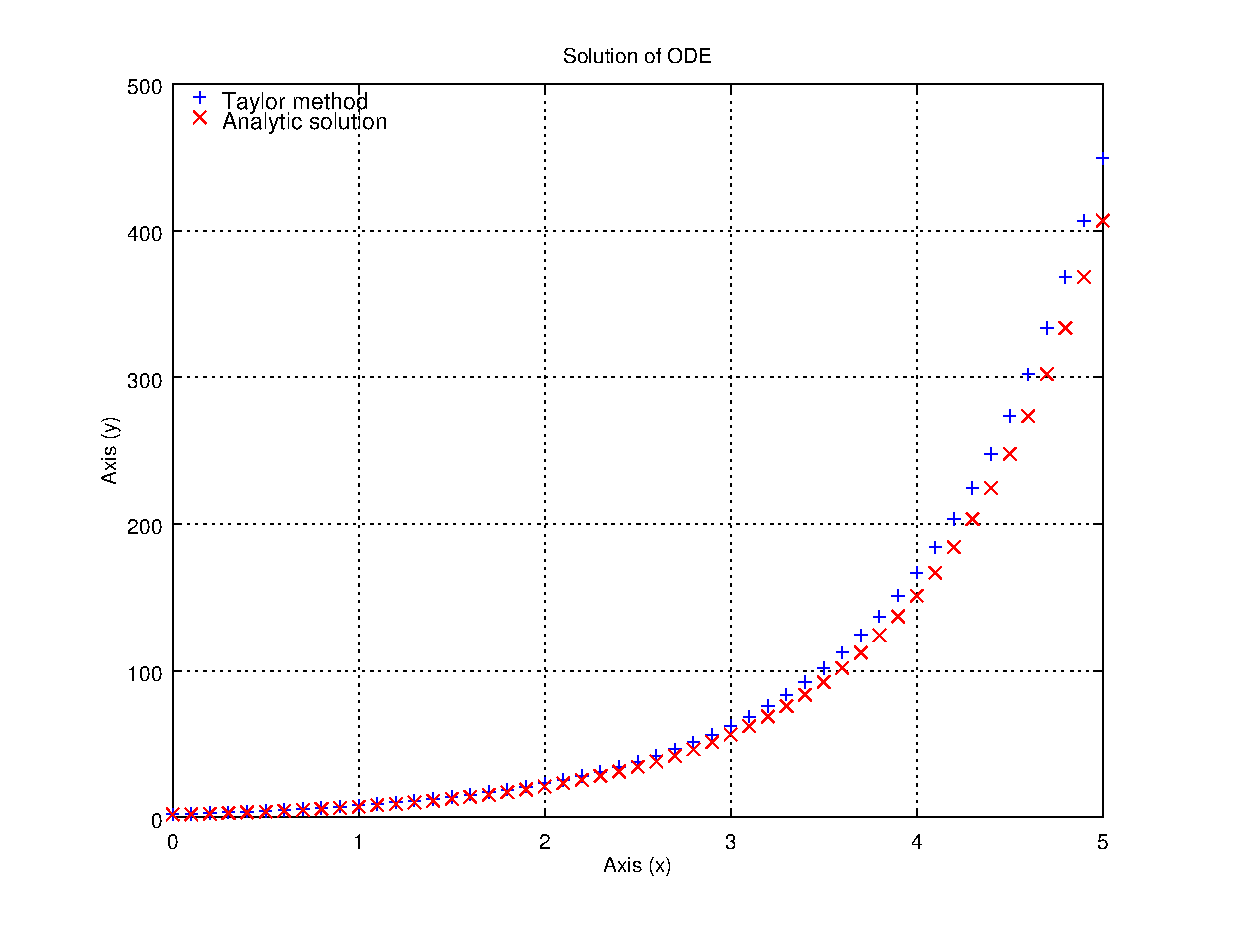
\includegraphics{plot1.eps}
		}
		\caption{Compara\c c\~ao solu\c c\~ao analitica e o m\'etodo de Taylor q = 3.}
	\end{figure}
\textbf{3. Quest\~ao:}\\

O c\'odigo a seguir se refere a implementa\c c\~ao do m\'etodo de Euler.
\verbatiminput{euler.txt}
\newpage
O c\'odigo a seguir se refere a resolu\c c\~ao do problema de valor inicial pelo m\'etodo de Euler.
\verbatiminput{testeEuler.txt}
	\begin{figure}[!h]
		\centering
		\label{fig2} 
		\resizebox{0.5\width}{!}{
			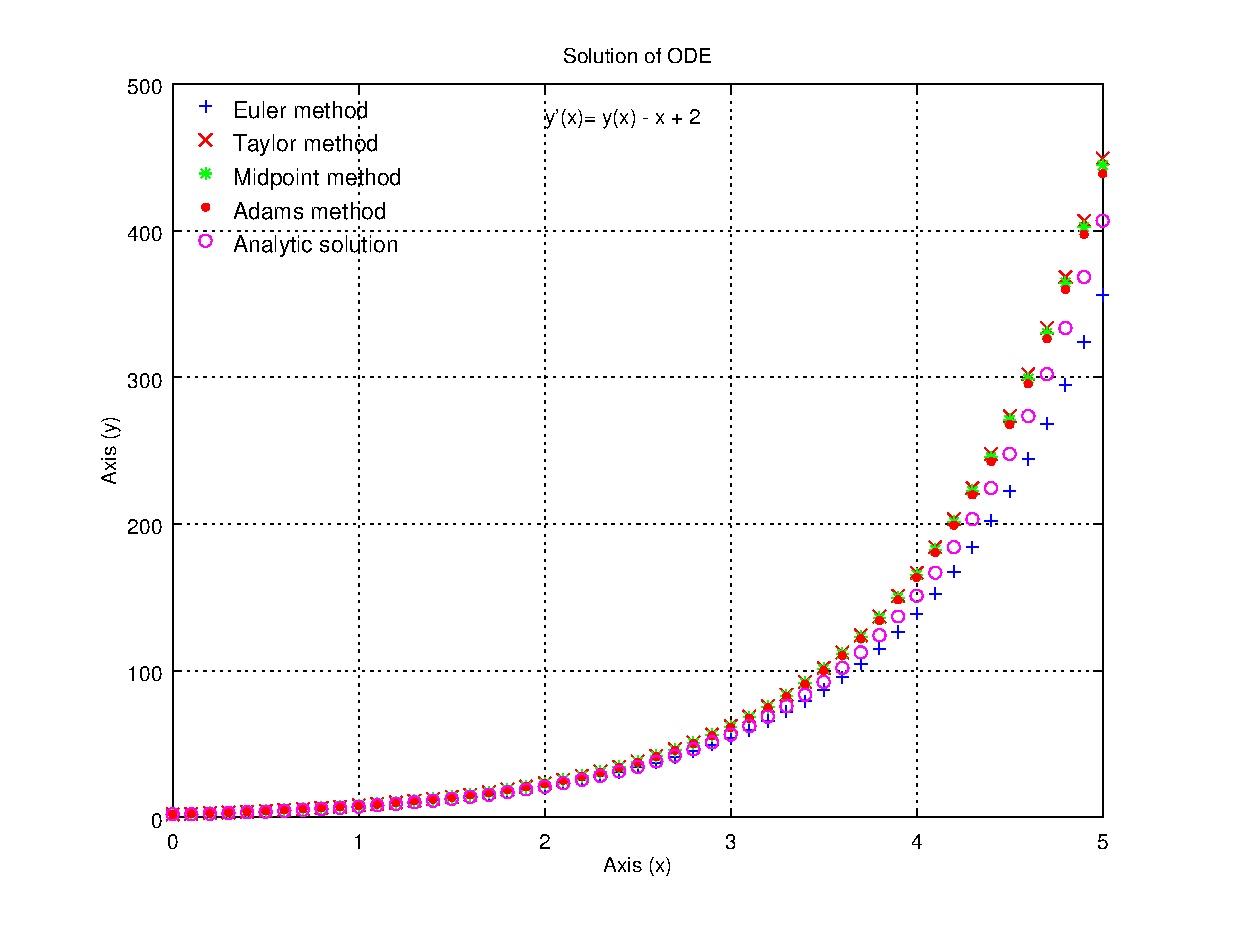
\includegraphics{plot2.eps}
		}
		\caption{Solu\c c\~ao do problema de valor inicial pelo m\'etodo de Euler.}
	\end{figure}
\newpage
Segue o c\'odigo modificado de teste.m com os m\'etodos de Euler e Taylor.
\verbatiminput{testeEulerTaylor.txt}
	\begin{figure}[!h]
		\centering
		\label{fig3} 
		\resizebox{0.5\width}{!}{
			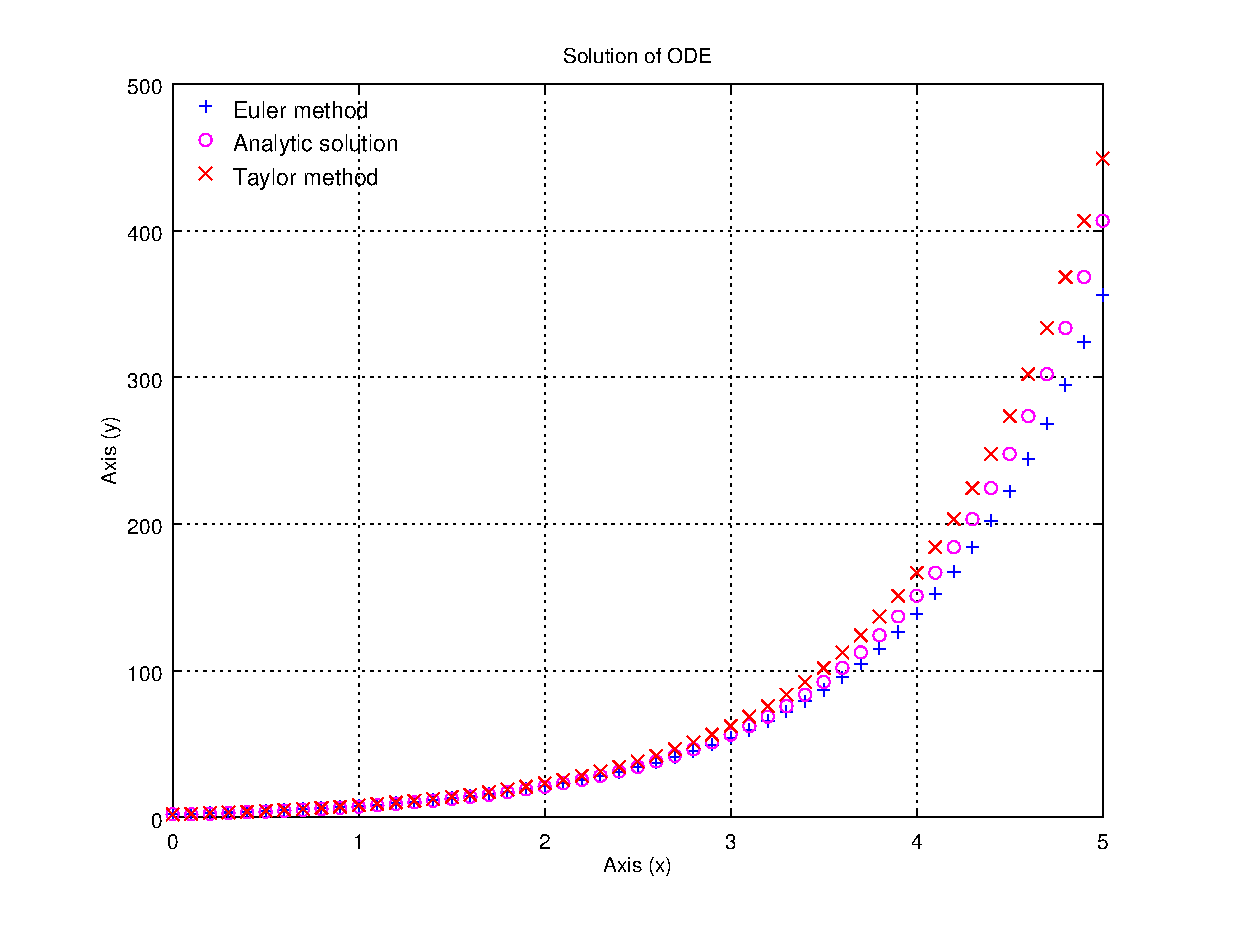
\includegraphics{plot3.eps}
		}
		\caption{Solu\c c\~ao do problema de valor inicial por Euler e Taylor.}
	\end{figure}
\textbf{4. Quest\~ao:}\\
A implementa\c c\~ao do m\'etodo de Adams Bashforth.
\verbatiminput{adams_bashforth.txt}

A implementa\c c\~ao do m\'etodo do ponto m\'edio.
\verbatiminput{ponto_medio.txt}
\textbf{5. Quest\~ao:}\\
Segue o c\'odigo para a quest\~ao 5.
\verbatiminput{teste3.txt}
Resultado da plotagem o passo 1.0 \'e n\~ao uma boa escolha.

	\begin{figure}[!ht]
		\centering
		\label{fig4} 
		\resizebox{0.5\width}{!}{
			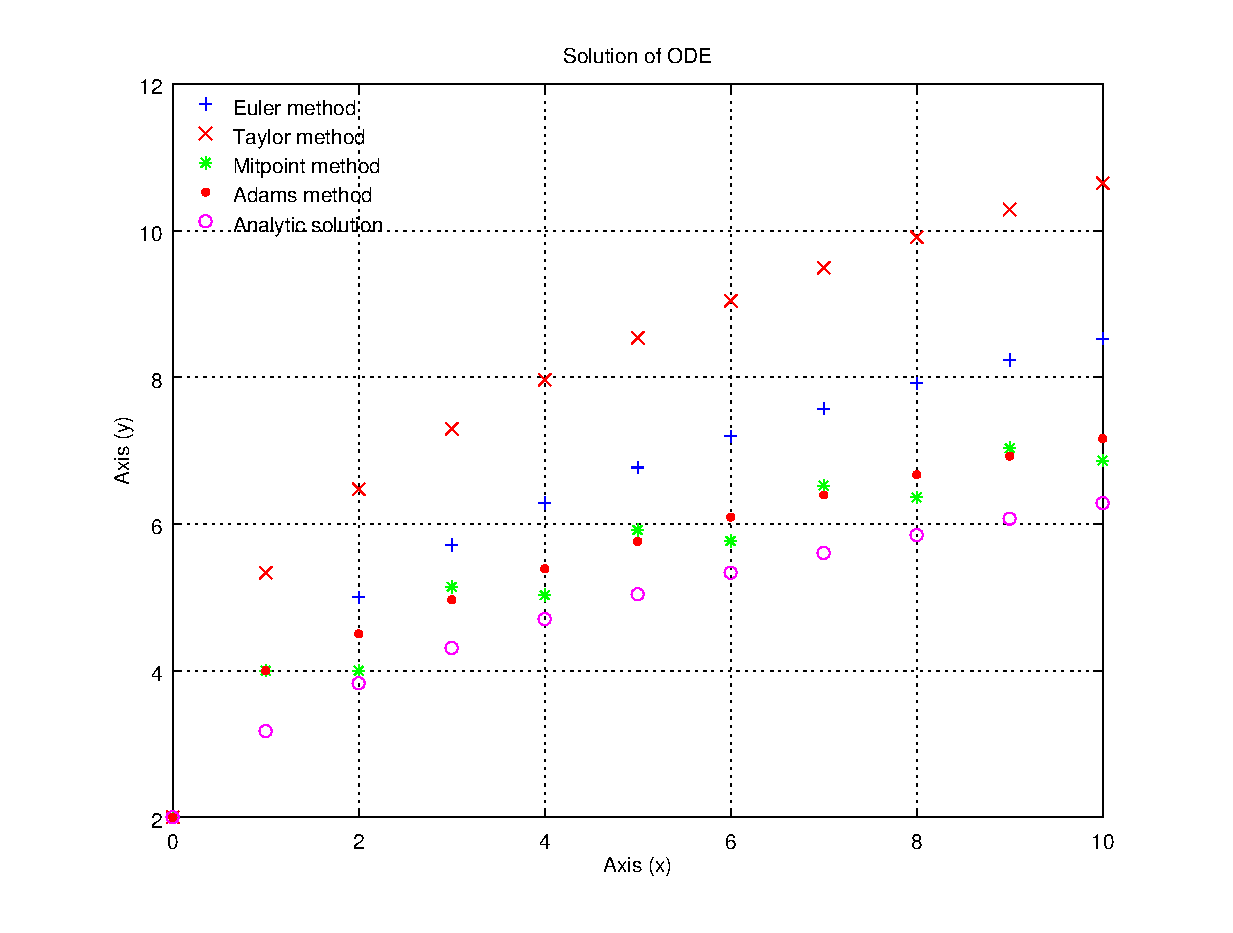
\includegraphics{plot4.eps}
		}
		\caption{Compara\c c\~ao entre os m\'etodos num\'ericos e a solu\c c\~ao anal\'itica.}
	\end{figure}
\pagebreak
\textbf{6. Quest\~ao:}\\

\begin{figure}[!ht]
	\resizebox{0.2\width}{!}{
	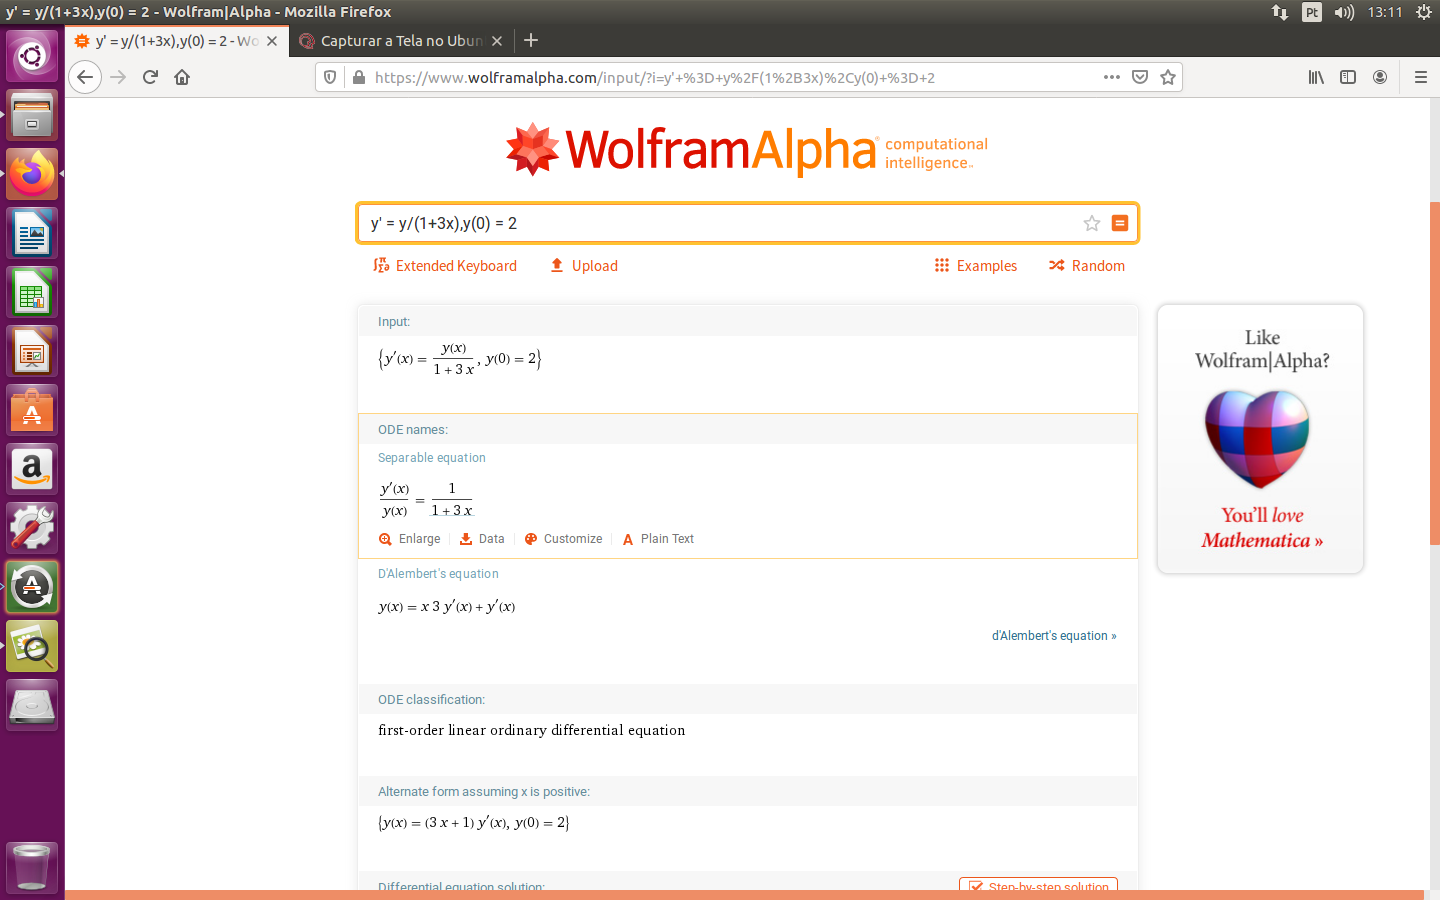
\includegraphics{alpha1.png}
	}
\end{figure}

\begin{figure}[!ht]
	\resizebox{0.2\width}{!}{
	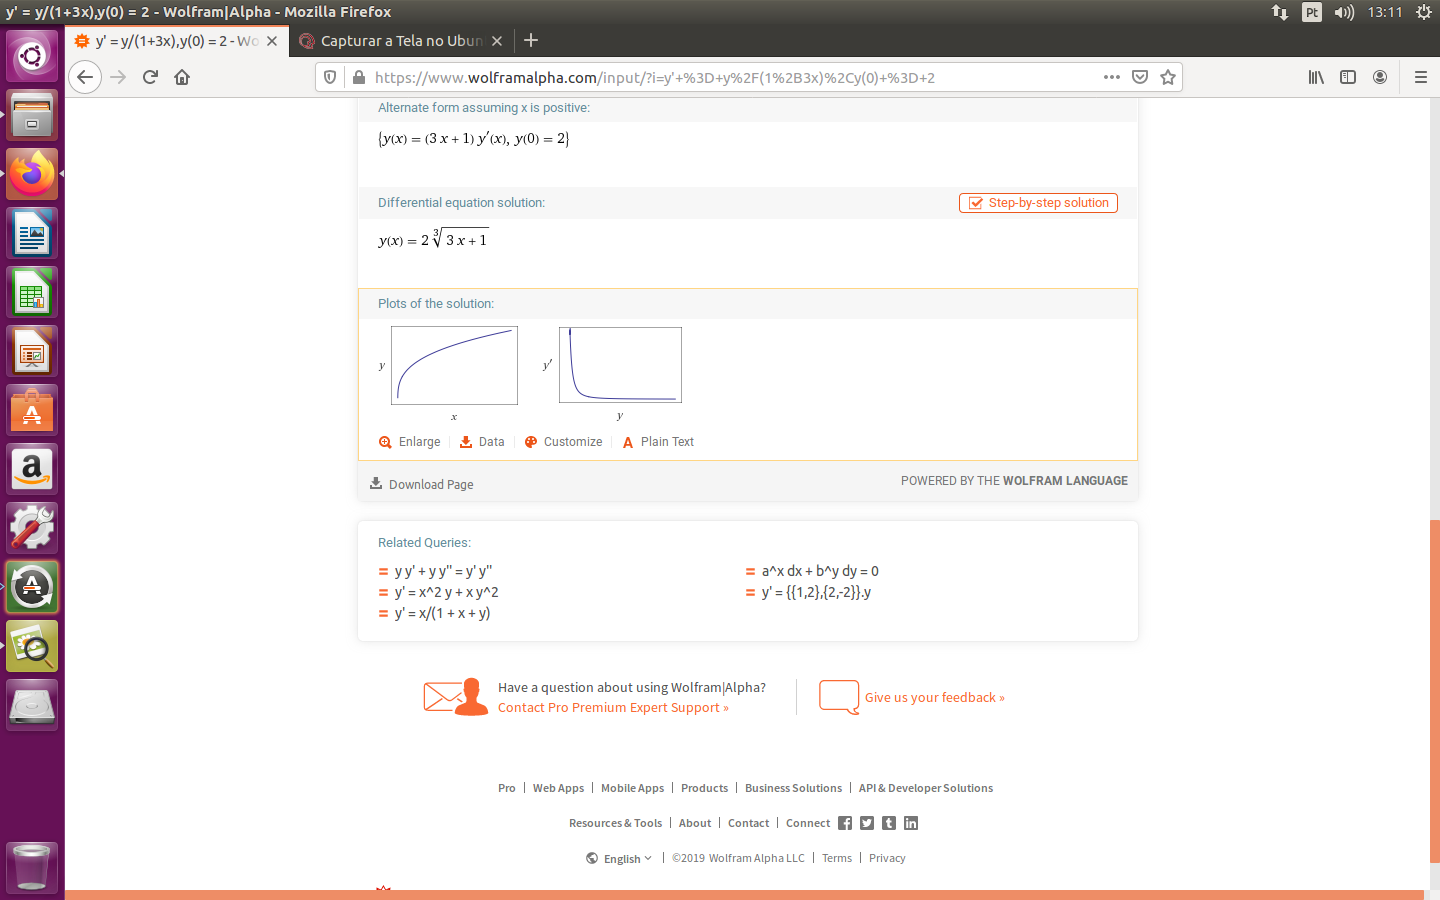
\includegraphics{alpha2.png}
	}
\end{figure}


\pagebreak
\textbf{7. Quest\~ao:}

a) Temos que o \textit{m\'etodo do ponto m\'edio} \'e dado por,
	\begin{align*}
		y_{n+2} &= y_{n} + 2hf_{n+1}\\
		&\mbox{ou}\\
		-y_{n} + 0y_{n+1} + y_{n+2} &= h(0f_n + 2f_{n+1} + 0f_{n+2}). 
	\end{align*}

Logo,
	\begin{align*}
		\alpha_{0} &= -1 \hspace{1cm}& \beta_{0} &= 0\\
		\alpha_{1} &=  0 \hspace{1cm}& \beta_{1} &= 2\\
		\alpha_{2} &=  1 \hspace{1cm}& \beta_{2} &= 0
	\end{align*}
segue que,
	\begin{align*}
		c_{0} &= \alpha_{0} + \alpha_{1} + \alpha_{2} &\Rightarrow \hspace{6pt} &c_{0} = -1 + 0 + 1 &\Rightarrow c_{0} = 0\\
		c_{1} &= \alpha_{1} + 2 \alpha_{2} -(\beta_{0} + \beta_{1} + \beta_{2}) &\Rightarrow \hspace{6pt}  &c_{1} = 0 + 2 -(0 + 2 + 0)
		&\Rightarrow c_{1} = 0 \\
		c_{2} &= \frac{1}{2!}(\alpha_{1} + 2^{2}\alpha_{2}) - \frac{1}{1!}(\beta_{1} + 2\beta_{2})	&\Rightarrow
		\hspace{6pt} &c_{2} = \frac{1}{2}(0 + 4) -(2 + 0) &\Rightarrow c_{2}  = 0 \\
		c_{3} &= \frac{1}{3!}(\alpha_{1} + 2^{3} \alpha_{2}) -\frac{1}{2!}(\beta_{1} + 2^{2}\beta_{2}) &\Rightarrow
		\hspace{6pt} &c_{3} = \frac{1}{6}(0 + 8) -\frac{1}{2}(2 + 0) &\Rightarrow c_{3} = \frac{1}{3}
	\end{align*}
	portanto, o \textit{m\'etodo do ponto m\'edio} possui ordem $q = 2$ com erro dado por $c_{3} = \frac{1}{3}.$ 

b) Temos que o \textit{m\'etodo de Simpson} \'e dado por,
	\begin{align*}
		y_{n+2} &= y_{n} + \frac{h}{3}[f_{n} + 4f_{n+1} + f_{n+2}]\\
		&\mbox{ou}\\
		-y_{n} + 0y_{n+1} + y_{n+2} &= h[\frac{1}{3}f_{n} + \frac{4} {3}f_{n+1} + \frac{1}{3} f_{n+2}]
	\end{align*}

Logo,
	\begin{align*}
		\alpha_{0} &= -1 \hspace{1cm}& \beta_{0} &= \frac{1}{3}\\
		\alpha_{1} &=  0 \hspace{1cm}& \beta_{1} &= \frac{4}{3}\\
		\alpha_{2} &=  1 \hspace{1cm}& \beta_{2} &= \frac{1}{3}
	\end{align*}
segue que,
	\begin{align*}
		c_{0} &= \alpha_{0} + \alpha_{1} + \alpha_{2} &\Rightarrow \hspace{6pt} &c_{0} = -1 + 0 + 1 &\Rightarrow
		\hspace{2pt} &c_{0} =
		0\\
		c_{1} &= \alpha_{1} + 2\alpha_{2} -(\beta_{0} + \beta_{1} + \beta_{2}) &\Rightarrow \hspace{6pt} &c_{1} = 0 +
		2 - (\frac{1}{3} + \frac{4}{3} + \frac{1}{3}) &\Rightarrow \hspace{2pt} &c_{1} = 0\\
		c_{2} &= \frac{1}{2!}(\alpha_{1} + 2^{2}\alpha_{2}) - \frac{1}{1!}(\beta_{1} + 2^{1}\beta_{2}) &\Rightarrow
		\hspace{6pt} &c_{2} = \frac{1}{2}(0 + 4)-(\frac{4}{3} + \frac{2}{3}) &\Rightarrow \hspace{6pt} &c_{2} = 0 \\
		c_{3} &= \frac{1}{3!}(\alpha_{1} + 2^{3}\alpha_{2}) - \frac{1}{2!}(\beta_{1} + 2^{2}\beta_{2}) &\Rightarrow
		\hspace{6pt} &c_{3} = \frac{1}{6}(0 + 8)-\frac{1}{2}(\frac{4}{3} + \frac{4}{3}) &\Rightarrow \hspace{6pt} &c_{3} = 0\\
		c_{4} &= \frac{1}{4!}(\alpha_{1} + 2^{4}\alpha_{2}) - \frac{1}{3!}(\beta_{1} + 2^{3}\beta_{2}) &\Rightarrow
		\hspace{6pt} &c_{4} = \frac{1}{24}(0 + 16)-\frac{1}{6}(\frac{4}{3} + \frac{8}{3}) &\Rightarrow \hspace{6pt}
		&c_{4} = 0\\
		c_{5} &= \frac{1}{5!}(\alpha_{1} + 2^{5}\alpha_{2}) - \frac{1}{4!}(\beta_{1} + 2^{4}\beta_{2}) &\Rightarrow
		\hspace{6pt} &c_{5} = \frac{1}{120}(0 + 32)-\frac{1}{24}(\frac{4}{3} + \frac{16}{3}) &\Rightarrow \hspace{6pt}
		&c_{5} = -\frac{1}{90}
	\end{align*}
portanto, a ordem do \textit{m\'etodo de Simpson} \'e q = 4 e o erro \'e $c_5 = -\frac{1}{90}.$
\\ \\
c) Temos que o \textit{m\'etodo de Adams-Moulton} \'e dado por,
	\begin{align*}
		y_{n+2} &= y_{n+1} + \frac{h}{12}[-f_{n} + 8f_{n+1} + 5f_{n+2}]\\
		&\mbox{ou} \\
		0y_{n} - y_{n+1} + y_{n+2} &= h[-\frac{1}{12}f_{n} + \frac{8}{12}f_{n+1} + \frac{5}{12}f_{n+2}]
	\end{align*} 

Logo,
	\begin{align*}
		\alpha_{0} &=  0 \hspace{1cm}& \beta_{0} &= -\frac{1}{12}\\
		\alpha_{1} &= -1 \hspace{1cm}& \beta_{1} &= \frac{8}{12}\\
		\alpha_{2} &=  1 \hspace{1cm}& \beta_{2} &= \frac{5}{12}
	\end{align*}
segue que,

	\begin{align*}
		c_{0} &= \alpha_{0} + \alpha_{1} + \alpha_{2} &\Rightarrow \hspace{6pt} &c_{0} = 0 -1 + 1 &\Rightarrow
		\hspace{2pt} &c_{0} =
		0\\
		c_{1} &= \alpha_{1} + 2\alpha_{2} -(\beta_{0} + \beta_{1} + \beta_{2}) &\Rightarrow \hspace{6pt} &c_{1} = -1 +
		2 - (-\frac{1}{12} + \frac{8}{12} + \frac{5}{12}) &\Rightarrow \hspace{2pt} &c_{1} = 0\\
		c_{2} &= \frac{1}{2!}(\alpha_{1} + 2^{2}\alpha_{2}) - \frac{1}{1!}(\beta_{1} + 2^{1}\beta_{2}) &\Rightarrow
		\hspace{6pt} &c_{2} = \frac{1}{2}(-1 + 4)-(\frac{8}{12} + \frac{10}{12}) &\Rightarrow \hspace{6pt} &c_{2} = 0 \\
		c_{3} &= \frac{1}{3!}(\alpha_{1} + 2^{3}\alpha_{2}) - \frac{1}{2!}(\beta_{1} + 2^{2}\beta_{2}) &\Rightarrow
		\hspace{6pt} &c_{3} = \frac{1}{6}(-1 + 8)-\frac{1}{2}(\frac{8}{12} + \frac{20}{12}) &\Rightarrow \hspace{6pt} &c_{3} = 0\\
		c_{4} &= \frac{1}{4!}(\alpha_{1} + 2^{4}\alpha_{2}) - \frac{1}{3!}(\beta_{1} + 2^{3}\beta_{2}) &\Rightarrow
		\hspace{6pt} &c_{4} = \frac{1}{24}(-1 + 16)-\frac{1}{6}(\frac{8}{12} + \frac{40}{12}) &\Rightarrow \hspace{6pt}
		&c_{4} = -\frac{1}{24}
	\end{align*}
portanto, a ordem do \textit{m\'etodo de Adams-Moulton} \'e q = 3 e o erro \'e $c_{4} = -\frac{1}{24}.$
\\ \\
d) Temos que o \textit{m\'etodo de Adams-Bashforth} \'e dado por,
	\begin{align*}
		y_{n+2} &= y_{n+1} + \frac{h}{2}[-f_{n} + 3f_{n+1}]\\
		&\mbox{ou} \\
		0y_{n} - y_{n+1} + y_{n+2} &= h[-\frac{1}{2}f_{n} + \frac{3}{2}f_{n+1}]
	\end{align*} 
Logo,
	\begin{align*}
		\alpha_{0} &=  0 \hspace{1cm}& \beta_{0} &= -\frac{1}{2}\\
		\alpha_{1} &= -1 \hspace{1cm}& \beta_{3} &= \frac{3}{2}\\
		\alpha_{2} &=  1 \hspace{1cm}& \beta_{2} &= 0
	\end{align*}
segue que,
	\begin{align*}
		c_{0} &= \alpha_{0} + \alpha_{1} + \alpha_{2} &\Rightarrow \hspace{6pt} &c_{0} = 0 -1 + 1 &\Rightarrow
		\hspace{2pt} &c_{0} =
		0\\
		c_{1} &= \alpha_{1} + 2\alpha_{2} -(\beta_{0} + \beta_{1} + \beta_{2}) &\Rightarrow \hspace{6pt} &c_{1} = -1 +
		2 - (-\frac{1}{2} + \frac{3}{2} + 0) &\Rightarrow \hspace{2pt} &c_{1} = 0\\
		c_{2} &= \frac{1}{2!}(\alpha_{1} + 2^{2}\alpha_{2}) - \frac{1}{1!}(\beta_{1} + 2^{1}\beta_{2}) &\Rightarrow
		\hspace{6pt} &c_{2} = \frac{1}{2}(-1 + 4)-(\frac{3}{2} + 0) &\Rightarrow \hspace{6pt} &c_{2} = 0 \\
		c_{3} &= \frac{1}{3!}(\alpha_{1} + 2^{3}\alpha_{2}) - \frac{1}{2!}(\beta_{1} + 2^{2}\beta_{2}) &\Rightarrow
		\hspace{6pt} &c_{3} = \frac{1}{6}(-1 + 8)- \frac{1}{2}(\frac{3}{2} + 0) &\Rightarrow \hspace{6pt} &c_{2} =
		\frac{5}{12}
	\end{align*}
portanto, a ordem do \textit{m\'etodo de Adams-Bashforth} \'e q = 2 e o erro \'e $c_{4} = -\frac{5}{12}.$
\\ \\
\textbf{8. Quest\~ao:}\\
a) Vamos analizar a estabilidade do m\'etodo dado por,
	\begin{align*}
		y_{n+2} - y_{n} &= 2hf_{n+1} \\
		&\mbox{ou}\\
		-y_{n} + 0y_{n+1} + y_{n+2} &= h(f_{n} + 2f_{n+1} + 0f_{n+2}
	\end{align*}
logo,
	\begin{align*}
		\alpha_{0} &= -1 \hspace{1cm}& \beta_{0} &= 0\\
		\alpha_{1} &=\hspace{8pt} 0 \hspace{1cm}& \beta_{1} &= 2\\
		\alpha_{2} &=\hspace{8pt} 1 \hspace{1cm}& \beta_{2} &= 0
	\end{align*}
segue que,
	\begin{align*}
		p(\varepsilon) &= \sum_{j=0}^{k}\alpha_{j}\varepsilon^{j} \\
		p(\varepsilon) &= \alpha_{0}\varepsilon^{0} + \alpha_{1}\varepsilon^{1} + \alpha_{2}\varepsilon^{2}\\
		p(\varepsilon) &= \varepsilon^{2} -1 \Rightarrow \varepsilon = \pm 1 
	\end{align*}
nota-se que as ra\'izes s\~ao simples e possuem o modulo menor ou igual 1. Portanto, o m\'etodo \'e est\'avel.

Vamos analisar a consist\^encia do m\'etodo,
	\begin{align*}
		c_{0} &= \alpha_{0} + \alpha_{1} + \alpha_{2} &\Rightarrow \hspace{6pt} &c_{0} = -1 + 0 + 1 &\Rightarrow
		\hspace{2pt} &c_{0} =
		0\\
		c_{1} &= \alpha_{1} + 2\alpha_{2} -(\beta_{0} + \beta_{1} + \beta_{2}) &\Rightarrow \hspace{6pt} &c_{1} = 0 +
		2 - (0 + 2 + 0) &\Rightarrow \hspace{2pt} &c_{1} = 0\\
		c_{2} &= \frac{1}{2!}(\alpha_{1} + 2^{2}\alpha_{2}) - \frac{1}{1!}(\beta_{1} + 2^{1}\beta_{2}) &\Rightarrow
		\hspace{6pt} &c_{2} = \frac{1}{2}(0 + 4)-(2 + 0) &\Rightarrow \hspace{6pt} &c_{2} = 0 
	\end{align*}
nota-se que como $c_{2} = 0$ o m\'etodo possue ordem $q \geq 1$. Portanto \'e consistente, por fim como \'e est\'avel e
consistente, logo, \'e convergente.

b) Vamos analisar a estabilidade do m\'etodo dado por,
	\begin{align*}
		y_{n+2} - y_{n+1} &= \frac{h}{3}(-2f_{n} + 3f_{n+1})\\
		&\mbox{ou}\\
		0y_{n} - y_{n+1} + 0y_{n+1} &= h(-\frac{2}{3} + f_{n+1} + 0f_{n+2})
	\end{align*}
logo,
	\begin{align*}
		\alpha_{0} &=\hspace{8pt} 0 \hspace{1cm}& \beta_{0} &= -\frac{2}{3}\\
		\alpha_{1} &= -1 \hspace{1cm}& \beta_{1} &= \hspace{8pt} 1\\
		\alpha_{2} &=\hspace{8pt} 1 \hspace{1cm}& \beta_{2} &= \hspace{8pt} 0
	\end{align*}
segue que,
	\begin{align*}
		p(\varepsilon) &= \sum_{j=0}^{k}\alpha_{j}\varepsilon^{j} \\
		p(\varepsilon) &= \alpha_{0}\varepsilon^{0} + \alpha_{1}\varepsilon^{1} + \alpha_{2}\varepsilon^{2}\\
		p(\varepsilon) &= \varepsilon^{2} -\varepsilon \Rightarrow p(\varepsilon) = \varepsilon(\varepsilon - 1)
		\Rightarrow \varepsilon = 0 \hspace{2pt} \mbox{ou} \hspace{2pt} 1
	\end{align*}
nota-se que todas as ra\'izes possuem m\'odulo menor ou igual a 1, al\'em disso a ra\'iz que tem m\'odulo igual a 1 \'e
simples, portanto, o m\'etodo \'e est\'avel.

Vamos analisar a consist\^encia do m\'etodo,
	\begin{align*}
		c_{0} &= \alpha_{0} + \alpha_{1} + \alpha_{2} &\Rightarrow \hspace{6pt} &c_{0} = 0 -1 + 1 &\Rightarrow
		\hspace{2pt} &c_{0} =
		0\\
		c_{1} &= \alpha_{1} + 2\alpha_{2} -(\beta_{0} + \beta_{1} + \beta_{2}) &\Rightarrow \hspace{6pt} &c_{1} = -1 +
		2 - (-\frac{2}{3} + 1 + 0) &\Rightarrow \hspace{2pt} &c_{1} = \frac{2}{3}
	\end{align*}
ordem do m\'etodo \'e $q = 0$, portanto o m\'etodo n\~ao \'e consistente. Logo, n\~ao \'e convergente.

c)
	\begin{align*}
		y_{n+2} - y_{n+1} &= \frac{h}{12}(-f_{n} + 8f_{n+1} + 4f_{n+2})\\
		&\mbox{ou}\\
		0y_{n} - y_{n+1} + 0y_{n+1} &= h(-\frac{1}{12}f_{n} + \frac{8}{12}f_{n+1} + \frac{4}{12}f_{n+2})
	\end{align*}
logo,
	\begin{align*}
		\alpha_{0} &=\hspace{8pt} 0 \hspace{1cm}& \beta_{0} &= -\frac{1}{12}\\
		\alpha_{1} &= -1 \hspace{1cm}& \beta_{1} &= \hspace{8pt} \frac{8}{12}\\
		\alpha_{2} &=\hspace{8pt} 1 \hspace{1cm}& \beta_{2} &= \hspace{8pt} \frac{4}{12}
	\end{align*}
Vamos analisar a estabilidade do m\'etodo,
segue que,
	\begin{align*}
		p(\varepsilon) &= \sum_{j=0}^{k}\alpha_{j}\varepsilon^{j} \\
		p(\varepsilon) &= \alpha_{0}\varepsilon^{0} + \alpha_{1}\varepsilon^{1} + \alpha_{2}\varepsilon^{2}\\
		p(\varepsilon) &= \varepsilon^{2} -\varepsilon \Rightarrow p(\varepsilon) = \varepsilon(\varepsilon - 1)
		\Rightarrow \varepsilon = 0 \hspace{2pt} \mbox{ou} \hspace{2pt} 1
	\end{align*}
portanto \'e est\'avel.
Vamos analisar a consist\^encia do m\'etodo,
	\begin{align*}
		c_{0} &= \alpha_{0} + \alpha_{1} + \alpha_{2} &\Rightarrow \hspace{6pt} &c_{0} = 0 -1 + 1 &\Rightarrow
		\hspace{2pt} &c_{0} =
		\hspace{6pt}0\\
		c_{1} &= \alpha_{1} + 2\alpha_{2} -(\beta_{0} + \beta_{1} + \beta_{2}) &\Rightarrow \hspace{6pt} &c_{1} = -1 +
		1 - (-\frac{1}{12} + \frac{8}{12} + \frac{4}{12}) &\Rightarrow \hspace{2pt} &c_{1} = \frac{11}{12}
	\end{align*}
ordem do m\'etodo \'e $q = 0$, portanto o m\'etodo n\~ao \'e consistente. Logo, n\~ao \'e convergente. 

d)
	\begin{align*}
		y_{n+2} - y_{n} &= \frac{h}{3}(-f_{n} + 4f_{n+1} + f_{n+2})\\
		&\mbox{ou}\\
		-1y_{n} + 0y_{n+1} + y_{n+1} &= h(\frac{1}{3}f_{n} + \frac{4}{3}f_{n+1} + \frac{1}{3}f_{n+2})
	\end{align*}
Vamos analisar a estabilidade do m\'etodo,
logo,
	\begin{align*}
		\alpha_{0} &= -1 \hspace{1cm}& \beta_{0} &= \frac{1}{3}\\
		\alpha_{1} &=\hspace{8pt} 0 \hspace{1cm}& \beta_{1} &= \hspace{8pt} \frac{4}{3}\\
		\alpha_{2} &=\hspace{8pt} 1 \hspace{1cm}& \beta_{2} &= \hspace{8pt} \frac{1}{3}
	\end{align*}
segue que
	\begin{align*}
		p(\varepsilon) &= \sum_{j=0}^{k}\alpha_{j}\varepsilon^{j} \\
		p(\varepsilon) &= \alpha_{0}\varepsilon^{0} + \alpha_{1}\varepsilon^{1} + \alpha_{2}\varepsilon^{2}\\
		p(\varepsilon) &= \varepsilon^{2} -1 \Rightarrow \varepsilon = \pm 1
	\end{align*}
portanto \'e est\'avel.\\
Vamos analisar a consist\^encia do m\'etodo,
	\begin{align*}
		c_{0} &= \alpha_{0} + \alpha_{1} + \alpha_{2} &\Rightarrow \hspace{6pt} &c_{0} = -1 + 0 + 1 &\Rightarrow
		\hspace{2pt} &c_{0} =
		\hspace{6pt}0\\
		c_{1} &= \alpha_{1} + 2\alpha_{2} -(\beta_{0} + \beta_{1} + \beta_{2}) &\Rightarrow \hspace{6pt} &c_{1} = 0 +
		2 - (\frac{1}{3} + \frac{4}{3} + \frac{1}{3}) &\Rightarrow \hspace{2pt} &c_{1} = 0\\
		c_{2} &= \frac{1}{2!}(\alpha_{1} + 2^{2}\alpha_{2}) - \frac{1}{1!}(\beta_{1} + 2^{1}\beta_{2}) &\Rightarrow
		\hspace{6pt} &c_{2} = \frac{1}{2}(0 + 2)-(\frac{4}{3} + \frac{2}{3}) &\Rightarrow \hspace{6pt} &c_{2} = -1 
	\end{align*}
ordem do m\'etodo \'e $q = 1$, portanto o m\'etodo \'e consistente. Como \'e est\'avel e consistente, portanto \'e
convergente. 

\textbf{9. Quest\~ao:}\\
Segue a implementa\c c\~ao do m\'etodo do previsor-corretor:
\verbatiminput{predCor9.m}

\textbf{10. Quest\~ao:}\\
Segue o c\'odigo do m\'etodo previsor-corretor, este \'e uma aplica\c c\~ao da quest\~ao 9, portanto, consulte o
c\'odigo  da quest\~ao 9 para uma explica\c c\~ao detalhada.
\verbatiminput{prevCor9.m}
\begin{figure}[!h]
	\centering
	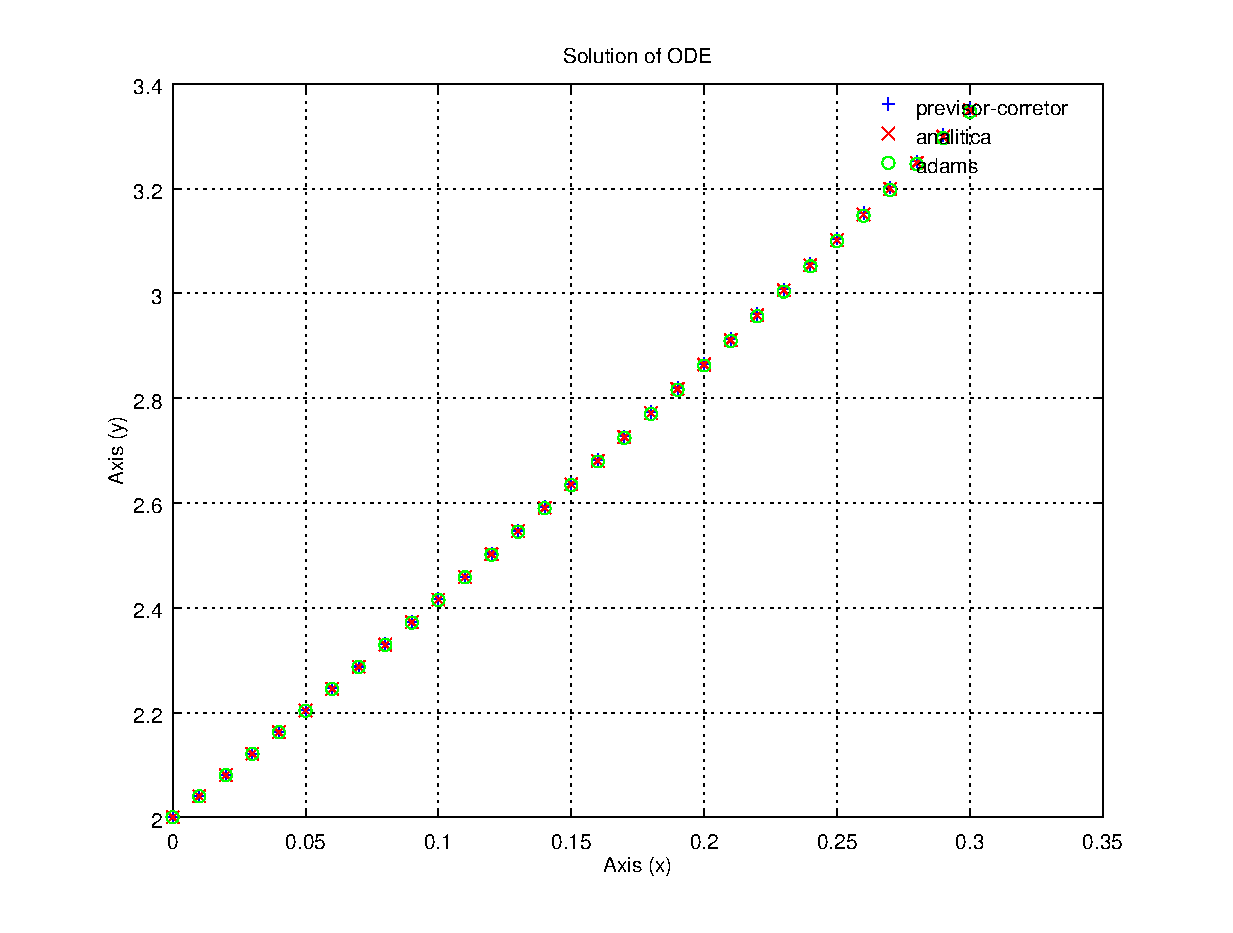
\includegraphics[width= 10cm]{plot6.eps}
\end{figure}
\end{document}


